\documentclass[serif,mathserif]{beamer}
\usepackage{amsmath, amsfonts, epsfig, xspace}
\usepackage{algorithm,algorithmic}
\usepackage{pstricks,pst-node}
\usepackage{multimedia}
\usepackage[normal,tight,center]{subfigure}
\setlength{\subfigcapskip}{-.5em}
\usepackage{beamerthemesplit}
\usetheme{lankton-keynote}

\author[Tejaswi KC, Raj Krishnan]{Group 11 \\ Tejaswi KC \quad Raj Krishnan \\ 140010020 \quad 140010007}

\title[PyAlpha\hspace{2em}\insertframenumber/\inserttotalframenumber]{PyAlpha: Interim Report}

\institute{Indian Institute of Technology, Bombay}

\begin{document}

  \maketitle

  \begin{frame}
    \frametitle{Tasks}
    \begin{itemize}
      \item Build a python module to handle the purchase and sale of stocks
       as per current prices on the share markets (Complete)
      \item Build a module to compute the quality of various alphas (weights
       for various stocks)
    \end{itemize}
  \end{frame}

  \begin{frame}
    \frametitle{Source Code}
    \begin{itemize}
      \item Hosted at https://github.com/raj-krishnan/PyAlpha
      \item Continuous Integration using Travis
      \item Coverage Testing using coveralls
      \end{itemize}
  \end{frame}

  \begin{frame}
    \frametitle{Dependencies}
    \begin{itemize}
      \item pandas
      \item peewee
      \item ystockquote
    \end{itemize}
  \end{frame}

  % \begin{frame}
  %   \frametitle{Installation}
  %   \begin{itemize}
  %     \item git clone https://github.com/raj-krishnan/PyAlpha.git
  %     \item cd PyAlpha
  %     \item pip install -r requirements.txt
  %     \item python setup.py install
  %     \item nosetests
  %   \end{itemize}
  % \end{frame}
  
  \begin{frame}
    \frametitle{Demo}
    \begin{figure}[h]
      \centering
      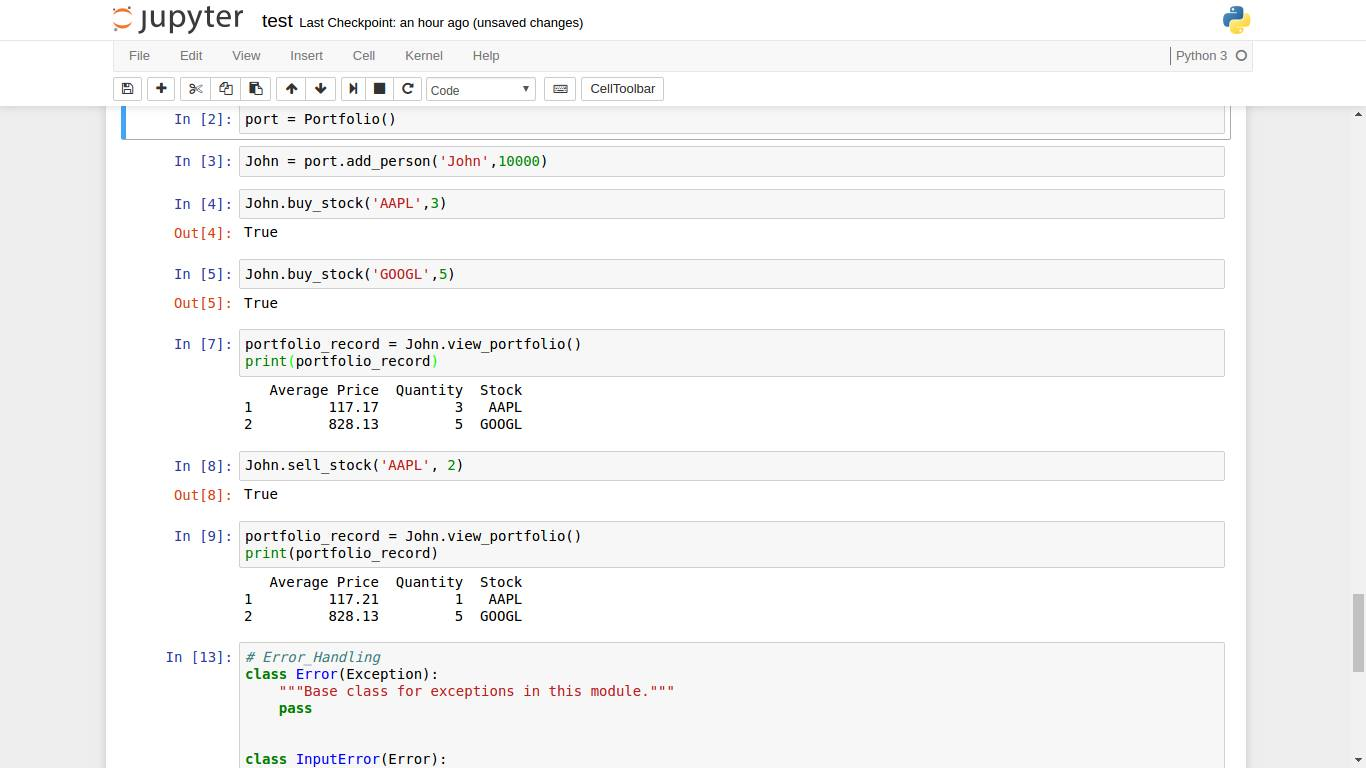
\includegraphics[width=\linewidth]{demo.png}
    \end{figure}
  \end{frame}

  \begin{frame}
    \frametitle{Plan for final submission}
    \begin{itemize}
      \item Complete specification 2 (module for Alpha testing)
      \item Provide complete documentation using sphinx
    \end{itemize}
  \end{frame}

  \begin{frame}
    \frametitle{Questions}
  \end{frame}

\end{document}
